%!TEX TS-program = xelatex
\documentclass[]{friggeri-cv}
\usepackage[UTF8]{ctex}
\usepackage{afterpage}
\usepackage{hyperref}
\usepackage{color}
\usepackage{xcolor}
\hypersetup{
    pdftitle={},
    pdfauthor={},
    pdfsubject={},
    pdfkeywords={},
    colorlinks=true,       % no lik border color
    allbordercolors=white    % white border color for all
}
\addbibresource{bibliography.bib}
\RequirePackage{xcolor}
\definecolor{pblue}{HTML}{0395DE}

\begin{document}
\header{闫}{博阳}
     
% Fake text to add separator      
\fcolorbox{white}{gray}{\parbox{\dimexpr\textwidth-2\fboxsep-2\fboxrule}{%
.....
}}

% In the aside, each new line forces a line break
\begin{aside}
  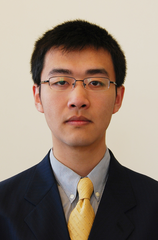
\includegraphics[scale=0.07]{img/boyang.png}
  \section{地址}
  天津市 南开区 宾水西道 华苑新城 竹华里 14-6-602
    ~
  \section{联系方式}
    \textbf{电话号码:} 13821579536
    \textbf{Skype:} yanboyang
    \textbf{微信:} yanboyang713
    ~
  \section{邮箱}
    \href{mailto:by932@uowmail.edu.au}{\textbf{by932@}\\uowmail.edu.au}
    \href{mailto:yanboyang713@gmail.com}{\textbf{yanboyang713@}\\gmail.com}
    ~
  \section{GitHub \& 个人网站}
    \href{https://github.com/yanboyang713}{github.com/yanboyang713}
    \href{http://www.yanboyang.com}{yanboyang.com}
    ~
  \section{程序语言}
    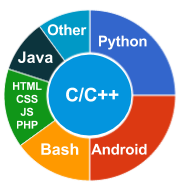
\includegraphics[scale=0.2]{img/programming.png}
    ~
\end{aside}

\section{教育背景}
\begin{entrylist}
  \entry
    {2018至今}
    {研究硕士 (计算机科学)}
    {伍伦贡大学(澳大利亚)}
    {软件测试方向\\
    主要课程: 软件测试, 研究方法, 大数据分析, 自然语言处理\\
    主要研究项目:跨语言感情倾向分析}
  \entry
    {2013 - 2017}
    {计算机科学本科​}
    {伍伦贡大学(澳大利亚)}
    {软件工程专业\\
    主要课程: C++ 程序语言, 算法与数据结构, 数据库系统, 系统安全, 多媒体课程(SDL, OPENGL), 操作系统, 计算机图形, Web开发, 软件开发方法与工具, 软件开发过程管理, 数学与统计学, 信息系统\\
    \emph{毕业项目名称: "基于网络的人力管理系统".}\\}
  \entry
    {2013}
    {学术英语}
    {伍伦贡大学语言学院(澳大利亚)}
    {主要课程: 听说读写}
  \entry
    {2011 - 2012}
    {工商管理本科}
    {中国矿业大学}
    
  \entry
    {2008 - 2011}
    {高中}
    {天津市津沽实验中学}
    {}
    
  \entry
    {2005 - 2008}
    {初中}
    {天津市津沽实验中学}
    
  \entry
    {2003 - 2005}
    {小学}
    {天津师范大学附属小学} 
    
  \entry
    {1999 - 2003}
    {小学}
    {新疆师范大学附属小学}  
    
\end{entrylist}
\newpage
\section{证书及获奖}
\begin{entrylist}
  \entry
    {2017}
    {最佳毕业项目奖}
    {伍伦贡大学(澳大利亚)}

  \entry
    {2017}
    {澳大利亚业余无线电操作证(标准)\\}
    {澳大利亚无线电协会(The Wireless Institute of Australia)}

  \entry
    {2016}
    {Ross a. Hull memorial Vhf-Uhf 无线电比赛\\}
    {澳大利亚无线电协会(The Wireless Institute of Australia)}
    {12名 Section A (模拟模式, 最好7天) 及 Section C (模拟模式, 最好两天)}

  \entry
    {2014}
    {澳大利亚业余无线电操作证(基础)\\}
    {澳大利亚无线电协会(The Wireless Institute of Australia)}
   
  \entry
    {2010}
    {天津市第92届中小学运动会 篮球第2名\\}
    {天津市}
    {高中男子B组及篮球2级运动员证}

\end{entrylist}

\section{培训课程}
\begin{entrylist}
  \entry
    {2012}
    {Intel innovation in EDUCATION}
    {Intel Learn Program (Technical and Community)}

\end{entrylist}

\section{奖学金}
\begin{entrylist}
  \entry
    {2014}
    {本科优秀学生奖学金}
    {伍伦贡大学(澳大利亚)}
    {\emph{25\% 学费减免}}
\end{entrylist}

\begin{aside}
  \section{Languages}
    \textbf{中文}
\includegraphics[scale=0.40]{img/5stars.png}
    \textbf{英语}
\includegraphics[scale=0.40]{img/4stars.png}
    ~
  \section{OS偏好}
    \textbf{GNU/Linux}
\includegraphics[scale=0.40]{img/5stars.png}
    \textbf{Unix}
\includegraphics[scale=0.40]{img/4stars.png}
    \textbf{MacOS}
\includegraphics[scale=0.40]{img/3stars.png}
    \textbf{Windows}
\includegraphics[scale=0.40]{img/1stars.png}
    ~
\end{aside}

\section{学术会议}
于2017年8月11号在悉尼参加Institute of Electrical and Electronics Engineers (IEEE)学术会议 (SC2017), 及展示本科毕业项目.

\section{业余活动}
我最主要的业余活动是业余无线电(amateur radio)。在2014年,
考取了第一个业余无线电操作证(foundation license)。刚开始只是为了练习英语通过与世界各地无线电爱好者交流。之后,目的慢慢开始变化,因为我发现业余无线电与计算机十分有联系,特别是数字模式。比如SSTV可以用于传输图片,D-STAR数字模式可以传输数据及数字语音。甚至国际空间站也有也有业余无线电中继站。从练习英语慢慢变成了关注研究业余无线电的技术部分,比如天线的结构,数字模式等。同时也参加一些业余无线电比赛并在澳大利亚ross a. Hull memorial vhf-uhf 比赛中获得名次。

\section{研究项目 \& 学校项目}
\subsection*{\textcolor{blue}{软件工程方面}}
\begin{entrylist}
  \entry
    {2018}
    {跨语言感情倾向分析测试\\}
    {伍伦贡大学(澳大利亚)}
    {}
\end{entrylist}

\begin{entrylist}
  \entry
    {2018}
    {使用Metamorphic测试方法测试文本对比工具\\}
    {伍伦贡大学(澳大利亚)}
    {使用Metamorphic测试方法测试DIFF utility的质量. 一共建立了10中 metamorphic relations.}
\end{entrylist}

\begin{entrylist}
  \entry
    {2017}
    {机器翻译工具测试\\}
    {伍伦贡大学(澳大利亚)}
    {使用metamorphic测试方法对Google, Bing 和有道翻译工具质量进行了对比及测试。\\\\ Github链接: \\{\small\url{https://github.com/yanboyang713/Metamorphic-Testing-of-Machine-Translation-Software.git}}}
\end{entrylist}

\begin{entrylist}
  \entry
    {2015}
    {针对游戏商店建立和使用各种UML图\\}
    {伍伦贡大学(澳大利亚)}
    {使用 UML 建立了use case diagram, class diagram, interaction diagram, context diagram 和 data flow diagram}
\end{entrylist}

\subsection*{\textcolor{blue}{多媒体方面}}
\begin{entrylist}
  \entry
    {2017}
    {使用OPENGL模拟创建一间房间\\}
    {伍伦贡大学(澳大利亚)}
    {使用OPENGL模拟创建了一间房间包括墙壁,地板,2幅画,桌椅及灯光等}
\end{entrylist}

\begin{entrylist}
  \entry
    {2017}
    {OPENGL 行星运动系统\\}
    {伍伦贡大学(澳大利亚)}
    {使用OPENGL建立了一个行星运动系统
    \\\\ Github链接: \\{\small\url{https://github.com/yanboyang713/openGLPlanetarySystem.git}}}
\end{entrylist}

\begin{entrylist}
  \entry
    {2016}
    {5th order低通Butterworth滤波器\\}
    {伍伦贡大学(澳大利亚)}
    {使用SDL库编写了一个5th order低通Butterworth滤波器,用于处理声音已减少噪音。 
     \\\\ Github链接: \\{\small\url{https://github.com/yanboyang713/butterworthFilter.git}}}
\end{entrylist}

\begin{entrylist}
  \entry
    {2016}
    {编写直方图均衡和灰度变换增强算法\\}
    {伍伦贡大学(澳大利亚)}
    {使用SDL编写直方图均衡和灰度变换增强算法,加强对比度和显示图片。
     \\\\ Github链接: \\{\small\url{https://github.com/yanboyang713/histogramEqualizationImage.git}}}
\end{entrylist}

\subsection{\textcolor{blue}{算法方面}}

\begin{entrylist}
  \entry
    {2017}
    {Tries数据结构\\}
    {伍伦贡大学(澳大利亚)}
    {使用Tries数据结构,用于文章词频统计,并排序。
     \\\\ Github链接: \\{\small\url{https://github.com/yanboyang713/tries-data-structure-count-unique-word-frequency.git}}}
\end{entrylist}

\begin{entrylist}
  \entry
    {2017}
    {商店服务模拟\\}
    {伍伦贡大学(澳大利亚)}
    {商店服务模拟drive by event 而不是 by time,主要使用了heap及queue。
     \\\\ Github Link: \\{\small\url{https://github.com/yanboyang713/simulate-shop-service.git}}}
\end{entrylist}

\subsection*{\textcolor{blue}{安全方面}}

\begin{entrylist}
  \entry
    {2017}
    {彩虹表\\}
    {伍伦贡大学(澳大利亚)}
    {使用c++编写彩虹表用于破解哈希算法。
    \\\\ Github链接: \\{\small\url{https://github.com/yanboyang713/rainbowTable.git}}}
\end{entrylist}

\subsection*{\textcolor{blue}{硬件方面}}

\begin{entrylist}
  \entry
    {2017}
    {刷卡系统\\}
    {伍伦贡大学(澳大利亚)}
    {使用Arduino, 树莓派, level shifter, LCD 控制器和 LCD 显示器制作考勤刷卡系统。在树莓派中,编写及使用Python实现树莓派与Arduino和Java后台通讯。并且使用I2C bus链接树莓派, Arduino 和 LCD控制器。使用Level shifter在I2C bus中转换不同电压。 RFID传感器与Arduino相连接。在Arduino中, 我写的c语言。}
\end{entrylist}

\begin{entrylist}
  \entry
    {正在做}
    {使用Google Home控制开关灯\\}
    {伍伦贡大学(澳大利亚)}
    {使用 NodeMCU 与 Google Home一起用于控制开关灯。}
\end{entrylist}

\subsection*{\textcolor{blue}{数据库方面}}

\begin{entrylist}
  \entry
    {2017}
    {MYSQL数据库\\}
    {伍伦贡大学(澳大利亚)}
    {为了本科毕业设计,设计及编写SQL用于管理MYSQL数据库。}
\end{entrylist}

\begin{entrylist}
  \entry
    {2017}
    {RDF Semantics 数据库\\}
    {伍伦贡大学(澳大利亚)}
    {使用 RDF semantics数据库记录电影信息。}
\end{entrylist}

\subsection*{\textcolor{blue}{网络方面}}

\begin{entrylist}
  \entry
    {2016}
    {个人博客\\}
    {伍伦贡大学(澳大利亚)}
    {使用Jekyll制作自己的blog。}
\end{entrylist}

\begin{entrylist}
  \entry
    {2014}
    {制作网站基于Drupal\\}
    {伍伦贡大学(澳大利亚)}
    {创建 Illawarra film Society 网站基于Drupal.}
\end{entrylist}

\section{个人评价}
积极向上,不断追求更好。对软件开发有很强的兴趣。从初中开始就一直喜欢计算机,在追求计算机中,虽然遇到过很多困难,但是一直没有放弃自己的追求。现在想通过找到一个软件开发的工作,来增加一些计算机软件的行业工作经验。在校期间,写过大量程序,基本上天天都写。个人感觉学习能力较强。

\section{推荐人信息}
\begin{itemize}
	\item George Zhou <zhiquan@uow.edu.au> 研究项目
	
	\item Jack Yang <jiey@uow.edu.au> 研究项目
	
	\item Eve Shaw <eve@uow.edu.au> 英语能力
	
	\item Mark Freeman <mfreeman@uow.edu.au> 本科毕业设计
	
	\item Casey Chow <caseyc@uow.edu.au> 计算机图形方面
	
	\item Tianbing Xia <txia@uow.edu.au> 基础编程及数据库
\end{itemize}



\begin{flushleft}
\emph{2018年10月17号}
\end{flushleft}
\begin{flushright}
\emph{闫博阳}
\end{flushright}

%%% This piece of code has been commented by Karol Kozioł due to biblatex errors. 
% 
%\printbibsection{article}{article in peer-reviewed journal}
%\begin{refsection}
%  \nocite{*}
%  \printbibliography[sorting=chronological, type=inproceedings, title={international peer-reviewed conferences/proceedings}, notkeyword={france}, heading=subbibliography]
%\end{refsection}
%\begin{refsection}
%  \nocite{*}
%  \printbibliography[sorting=chronological, type=inproceedings, title={local peer-reviewed conferences/proceedings}, keyword={france}, heading=subbibliography]
%\end{refsection}
%\printbibsection{misc}{other publications}
%\printbibsection{report}{research reports}
\end{document}
